\documentclass[a4paper]{article}
\usepackage[francais]{babel}
\usepackage[utf8]{inputenc}

\usepackage{graphicx}
\usepackage{fancyhdr}
\usepackage{lastpage}
\usepackage{amsmath}
\usepackage{xspace}
\usepackage{textcomp}

\usepackage{hyperref}

\usepackage[top=30mm, bottom=30mm, left=25mm, right=25mm]{geometry}

\pagestyle{fancy}

\usepackage{helvet}
\usepackage{bbm}

\usepackage{verbatim}
\usepackage{amsmath}
\usepackage[table]{xcolor}
\definecolor{bleugris}{rgb}{.2,.4,.5}

\definecolor{colKeys}{rgb}{0,0,1} 
\definecolor{colIdentifier}{rgb}{0,0,0} 
\definecolor{colComments}{rgb}{0,0.5,1} 
\definecolor{colString}{rgb}{0.6,0.1,0.1} 

\usepackage{listings}

% Permet l'ajout de code par insertion du fichier le contenant
% Les arguments sont :
% $1 : nom du fichier à inclure
% $2 : le type de langage (C++, C, Java ...)
\newcommand{\addCode}[2]{%

  % Configuration de la coloration syntaxique du code
  \definecolor{colKeys}{rgb}{0,0,1}
  \definecolor{colIdentifier}{rgb}{0,0,0}
  \definecolor{colComments}{rgb}{0,0.5,1}
  \definecolor{colString}{rgb}{0.6,0.1,0.1}

  % Configuration des options 
  \lstset{%
    language = #2,%
    identifierstyle=\color{colIdentifier},%
    basicstyle=\ttfamily\scriptsize, %
    keywordstyle=\color{colKeys},%
    stringstyle=\color{colString},%
    commentstyle=\color{colComments},%
    columns = flexible,%
    %tabsize = 8,%
    showspaces = false,%
    numbers = left, numberstyle=\tiny,%
    frame = single,frameround=tttt,%
    breaklines = true, breakautoindent = true,%
    captionpos = b,%
    xrightmargin=10mm, xleftmargin = 15mm, framexleftmargin = 7mm,%
  }%
    \begin{center}
    \lstinputlisting{#1}
    \end{center}
}

\newcommand{\nTitle}[1]{%
	\clearpage
	\vspace*{\fill}		%
	\begin{center}	%
		\part{#1}		%
	\end{center}
	\vspace*{\fill}		%
	\clearpage
}

\newenvironment{nAbstract} 		%
{ 								%
	\newpage 					% 
	\vspace*{\fill}				%
	\begin{center}			 	%
		\begin{abstract}		%
}{								%
		\end{abstract}			%
	\end{center}				%
	\vspace*{\fill}				%
	\newpage					%
}


\newcommand{\nClass}[1]{{\color{bleugris}{\textsl{\textbf{#1}}}}}
\newcommand{\nParameter}[1]{{\color{gray}{\textbf{#1}}}}
\newcommand{\nMethod}[1]{{\color{gray}{\textbf{#1}}}}
\newcommand{\nConstant}[1]{\texttt{\uppercase{#1}}}
\newcommand{\nKeyword}[1]{\textsl{\textbf{#1}}}

\graphicspath{{../SourcesMatlab/}}

% Conversion nombres arabes / romain
\makeatletter
\newcommand{\rmnum}[1]{\romannumeral #1}
\newcommand{\Rmnum}[1]{\expandafter\@slowromancap\romannumeral #1@}
\makeatother

\setlength{\headheight}{14pt}

\fancyhf{}


\makeatletter
\def\clap#1{\hbox to 0pt{\hss #1\hss}}%
\def\ligne#1{%
\hbox to \hsize{%
\vbox{\centering #1}}}%
\def\haut#1#2#3{%
\hbox to \hsize{%
\rlap{\vtop{\raggedright #1}}%
\hss
\clap{\vtop{\centering #2}}%
\hss
\llap{\vtop{\raggedleft #3}}}}%
\def\bas#1#2#3{%
\hbox to \hsize{%
\rlap{\vbox{\raggedright #1}}%
\hss
\clap{\vbox{\centering #2}}%
\hss
\llap{\vbox{\raggedleft #3}}}}%
\def\maketitle{%
\thispagestyle{empty}\vbox to \vsize{%
\vfill
\vspace{1cm}
\begin{flushleft}
\usefont{OT1}{ptm}{m}{n}
\huge \@title
\end{flushleft}
\par
\hrule height 4pt
\par
\begin{flushright}
\usefont{OT1}{phv}{m}{n}
\Large \@author
\par
\end{flushright}
\vspace{1cm}
\vfill
\vfill
\bas{}{\@blurb \vspace{1cm}}{}
}%
\cleardoublepage
}
\def\date#1{\def\@date{#1}}
\def\author#1{\def\@author{#1}}
\def\title#1{\def\@title{#1}}
\def\blurb#1{\def\@blurb{#1}}
\author{}
\title{}
\blurb{}
\makeatother


\usepackage{hyperref}
\hypersetup{
colorlinks=false, % bool: Liens colorés
pdfborder={0 0 0} % Ne pas encadrer les liens
}

\usepackage[final]{pdfpages}
\usepackage{rotating}
\usepackage{eurosym}
\usepackage{lscape}
\usepackage{float}
\usepackage{color}
\usepackage{colortbl}
\usepackage{array}
\usepackage[printonlyused]{acronym}
\usepackage{url}

% définir les commandes ici

% s'il y a beaucoup de commandes et de packages à inclure n'h&ésitez pas
% à mettre tout ça dans un fichier include.tex et l'inclure
% \input{include.tex}

\lhead{Synthèse bibliographique}
\rhead{
\includegraphics [width=1.5cm]{insa-couleur.jpg}}
\rfoot{\thepage\ de \pageref{LastPage}}



\begin{document}
\title{Nettoyage des données en présence de données de référence}
\author{Elisa ABIDH, Julien LEVESY,Armand ROSSIUS}

%------------------------------------- Page de titre
\maketitle
%\begin{titlepage}
%~

%\vfill
%\begin{Large}
%Septembre 2011
%\end{Large}
%\vfill
%\end{titlepage}
%----------------------------------------------------

%--------------------------------- Table des matières
\newpage
\tableofcontents
\newpage
%----------------------------------------------- Plan
\subsection {Enjeux de la qualité de données}
Depuis plusieurs années la gestion des données est devenue cruciale pour les entreprises, le volume de données stockées et échangées augmentent, ce qui confronte les entreprise à la problématique de comment stocker les données et pouvoir y accéder facilement, on parle alors de  "Data Management" ou gestion des données.\\ Que ce soit pour des raisons légales, des besoins opérationnelles ou pour des choix stratégiques la gestion de l'information est importante.  Au sein d'une entreprise beaucoup d'activités et fonctions sont concernées :
\begin{itemize}
\item[-] La gestion d’activité optimale pour répondre à la demande : demande une maitrise de l’information.
\item[-] Toutes les fonctions des entreprises sont gérées par le SI
\item[-] Les données sont un flux présent dans toutes les entreprises
\item[-] Les dirigeants : parce que les décisions, le plan stratégique nécessite de l’information
\item[-] Les responsables opérationnels : ils traitent de l’information pour pouvoir gérer au mieux les problèmes. 
\item[-] Marketing : données sur les fournisseurs, les clients, les concurrents, les marchés
\item[-] Les collaborateurs opérationnels : approvisionner le stock, lister des interventions sur une machine, nom des pièces changées
\end{itemize}
On comprend que la qualité des données gérer par le SI est importante pour répondre aux attentes du client mais aussi pour gérer de manière optimale l'entreprise. Cependant l'entreprise va rencontrer plusieurs difficultés pour répondre à cette problématique de  qualité de données : 
\begin{itemize}
\item[-]Détecter la mauvaise qualité des données.
\item[-]Trop de données car beaucoup de données inutiles. 
\end{itemize}
Avant de répondre à cette problématique il est légitime de se poser la question : "Qu'est ce qu'une donnée de qualité ? "
D'après le livre de Christophe Brasseur \cite{Brasseur} la qualité ne se résume pas à une donnée juste, c'est une condition nécessaire mais non suffisante. Il est difficile de donner une définition précise de cette notion, cependant on peut dégager plusieurs axes pour juger de la qualité des données : qualité du contenu, accessibilité, flexibilité, sécurité.
\begin{enumerate}
\item {Qualité du contenue}
\begin{itemize}
\item[-]Justesse de l’information : en phase avec la réalité
\item[-]Adéquation aux besoins : réponds aux besoins réels
\item[-]Facilité d'interprétation : pas d'ambiguïté(abrévation,unités), compréhensible.
\end{itemize}
\item {Accessibilité}
\begin{itemize}
\item[-]Disponibilité : disponible quand on en a besoin
\item[-]Facilité d’accès : ergonomie des applications.
\end{itemize}
\item {Flexibilité}
\begin{itemize}
\item[-]Evolutivité : définition et codification de la donnée (pas de remise en cause) 
\item[-]Cohérence avec d’autres sources (identifier les données partagées), 
\item[-]Possibilité de traduction.
\end{itemize}
\item {Sécurité}
Protéger l’information des menaces accidentelles et des attaques malveillantes
\begin{itemize}
\item[-]Confidentialité 
\item[-]Fiabilité 
\item[-]Traçabilité
\item[-]Intégrité des données.
\end{itemize}
\end{enumerate}



\section{Démarche}

N'étant pas, par notre formation et nos affinités, des personnes ayant une grande connaissance des problématiques de gestion de données d'entreprise au sein d'un SI, nous avons décidé d'adopter une démarche d'ingénieur "ingénu"  vis à vis du problème posé.\\
Par cela, nous entendons avoir une démarche progressive et critique vis à vis du vaste problème qu'est la qualité des données au sein d'un SI. Ce sujet étant extrêmement vaste et mal défini, nous ne souhaitons pas nous fermer de portes dans notre raisonnement.\\
De plus, nous souhaitons réellement avoir une approche qui permette de distinguer la réalité des intérêts technologiques des arguments commerciaux de bas étage, ces derniers étant plus que mis à contribution  compte tenu du battage médiatique effectué autour de la problématique de la qualité des données. Nous tâcherons de passer outre ces aspects.\\
Ainsi, dans un premier temps, nous allons nous atteler à définir le domaine de la qualité des données, pour ensuite essayer d'effectuer un aperçu des approches possibles de la problématique de qualité des données, pour enfin déboucher sur le management des données de référence, son fonctionnement, son implémentation dans un SI d'entreprise et les différents challenges que ce type de service pose au sein d'une entreprise.\\
De cette manière nous espérons fournir un aperçu complet et critique de cette technologie. 
\section{Une réponse : le master data management}

\subsection{Présentation du procédé et objectifs} 

Le Master Data Management, traduit en français par Gestion des données de références, est une discipline des technologies de l'information ayant pour objectif de définir des concepts et méthodes visant à établir au sein d'un système d'informations un schéma de base de données de références considérées comme fiables.\\
Outre cela, le Master Data Management englobe aussi les disciplines d'intégration, d'exposition et d'utilisation de ces données de références au sein d'un système d'information d'entreprise, autant du coté opérationnel que analytique.\\
Ce procédé, permet de répondre en partie à la problématique de la qualité des données, en définissant un cadre de données dites de références, considérées comme sures, et limite ainsi, l'entropie des données intégrées aux entrepôts de données, mais n'effectue pas à proprement parler de nettoyage des données, thème qui sera abordé dans la suite de la synthèse\\
A la différence d'un "simple" nettoyage instancié une ou plusieurs fois dans le parc de données de l'entreprise, le Master Data Management inscrit une démarche de qualité de données sur le long terme.\\

L'hypothèse de base est la suivante : \textit{"En assurant la qualité sur les données de références, on limite les erreurs lors de l'alimentation et l'exploitation de l'entrepôt de données"}\\

\subsection{Données, de quoi parle-t-on ?}

\subsubsection{Donnée Transactionnelle}

Chaque opération effectuée dans l'entreprise génère des données. Par exemple lors d'un achat
les données générées sont : date de l'achat, quantité de produit acheté, montant transaction et cie...
Des bases de données basées sur de l'OLTP sont utilisées pour la gestion de ce genre de transactions.
Des techniques de gestion de ces données existent, pour gérer ces données, notamment via le nettoyage par données de références, que nous aborderons dans la suite de cette synthèse.

\subsubsection{Donnée Analytique}

Les données analytiques sont générées à partir des bases de données transactionnelles et des bases de données de références.\\
Il s'agit ici de traiter des données transactionnelles sur le plus ou moins long terme, les traitements et l'exploitation étant orientés en fonction de grands axes.\\
Deux principales approches se distinguent dans le monde de la business intelligence :
\begin{itemize}
\item Modélisation OLAP : Transformation des entrepôts de données d'entreprises en "hypercubes", permettant une exploitation facilitée (création de rapports, tableaux d'indicateurs...)
\item Datamining : Recherche de regroupements de tuples en fonction de leurs attributs, dans les bases de données d'entreprise, de façon à effectuer de l'analyse prédictive entre-autres. Un exemple concret est le "pattern" de navigation internet d'un utilisateur moyen, permettant au final de "prédire" quelle sera sa prochaine étape de navigation
\end{itemize}

\subsubsection{Données de références, késako ? }

Les données de références sont un sous ensemble des données opérationnelles, considérées comme données de support pour les différentes opérations d'alimentation ou d'exploitation des données du SI. Elles possèdent une certaine constance dans le temps, qui n'est cependant pas une invariance, ces données pouvant être modifiées, complétées voire étendues. Ce sont ces mêmes données qui vont définir les axes d'exploration, d'exploitation et d'analyse.\\
On différencie trois grandes catégories de données de références.

\begin{itemize}
\item Produit : Chaque entreprise possède une quantité de référence produits, qui peuvent êtres transversaux à plusieurs secteurs de l'entreprise. Typiquement, un produit pourra être référencé par une documentation technique issue d'un bureau d'étude, une opération de vente  ou encore un référentiel fournisseur. L'unicité devra donc être assurée sur l'ensemble des entrées dans ce domaine.
\item Tiers : De façon similaire, les "tiers" d'entreprises sont aussi considérés comme données de références. Par tiers nous entendons toute personne ou entité ayant une interaction possible avec le système d'information, typiquement un collaborateur, un client ou encore un fournisseur.
\item Finance  : Les données de finances sont des informations critiques pour le fonctionnement de l'entreprise, obligatoire en ce qui concerne n'importe quel aspect légal et primordial en ce qui concerne le pilotage des activités. Ces deux approches sont intégrées à la gestion de données de références.
\end{itemize}

Une question demeure en suspends... Quand une donnée normale peut être considérée comme donnée de référence ?\\
En effet, la simple différenciation basée sur le fait qu'une donnée est transactionnelle ou non, peut dans certains cas se révéler mise en défaut.\\
Prenons pour exemple une opération de vente du produit P1 à Mr M enregistrée par une application opérationnelle, cela se traduit par une entrée dans la table vente de l'entrepôt en relation avec les données de références produit...\\
Maintenant, est-il possible de considérer le fait que l'acheteur constitue en lui même une donnée de référence ? Mieux encore, la quantité de produit P1 vendue à ce client peut à son tour être considérée comme une donnée de référence...\\
Cet exemple met en évidence que la frontière entre une donnée de référence ou une donnée standard n'est pas clairement définie aux yeux de tous. Clairement, en suivant la logique précédente, la totalité de l'entrepôt de données de l'entreprise peut être considérée comme donnée de référence.\\
Plusieurs pistes pour répondre à cette question : \\

\begin{itemize}
\item Donnée de support pour l'alimentation et l'exploitation de l'entrepôt de données de l'entreprise. Dimensions d'analyse lors de l'exploitation en OLAP par exemple.
\item Objets métiers partagés entre plusieurs applications de l'entreprise
\end{itemize}

\subsubsection{Pourquoi définir un parc de données de références de qualité ?}

Comme expliqué auparavant, les données de références au sein d'un système d'information servent d'axes d'exploitation et d'analyse. Ainsi chaque opération effectuée au sein de ce dernier est obligatoirement rattachée à une ou plusieurs données de référence. Si celles-ci sont corrompues, fausses, non unifiées, le risque d'augmentation de l'entropie au sein de l'entrepôt s'en trouve décuplé.\\
Par exemple, dans un repère orthogonal de dimension 3, caractérisé par les axes (x,y,z), positionner un point aux coordonnées (1,2,3) est quelque chose de relativement aisé, si et seulement si les valeurs 1,2 et 3 des axes sont garanties comme unique.
Émettons alors l'hypothèse que non, les valeurs présentes ne sont pas uniques... La question de l'insertion d'un point aux coordonnées (1,2,3) se révèle alors beaucoup plus complexe, quelle valeur choisir ? \\ 
Nous nous retrouverions automatiquement en face d'un parc de n valeurs possédant toutes les caractéristiques (1,2,3) ... différentes !\\
Autre chose, recherchons maintenant tous les points résolvant la condition y = 2, ce qui peut s'apparenter à la recherche de caractéristique commune pour des entrées produit dans le cas réel.
La encore, si "2 possède plusieurs valeurs" dans le repère, la tâche de regroupement s'avère encore plus complexe.\\
Imaginez les risques, sur une base de données opérationnelles, avec un nombre de tuples extrêmement grand.\\

\section{Fonctionnement du M.D.M. dans un système d'information d'entreprise}

\subsection{Principe de fonctionnement}

Nous l'avons vu, il est indispensable d'avoir un parc de données de références de qualité si l'on souhaite pouvoir exploiter correctement ces données dans les applications opérationnelles du S.I., et ainsi maintenir une certaine cohérence. Cette cohérence est également indispensable pour l'exploitation de ces données par le système de Business Intelligence de l'entreprise.\\

\subsubsection{Fonctionnement de base d'un système de Master Data Management}

Afin d'expliquer clairement le fonctionnement d'un système de Master Data Management, il convient de présenter le fonctionnement d'un S.I. sans la présence de M.D.M.
Sans système de M.D.M, chaque application du système d'information possède une base de données qui lui est propre, et y accède de manière informelle.
Les modifications, créations et suppression de données ne sont donc pas tracées. De nombreux problèmes de cohérence et de corruption de données sont présents de par la présence de sources de données multiples, de données incomplètes, erronées ou incohérentes.\\\\

L'objectif du Master Data Management est de fournir une base de données unique et unifiée  pour l'ensemble des applications opérationnelles du S.I.\\
Ainsi, l'ensemble des applications du S.I. partage les mêmes informations, éliminant ainsi les problèmes de cohérence et de corruption des données.\\
La maintenance des données ne s'effectue donc qu'à un seul endroit, et est donc simplifiée. Le système de M.D.M. distribue ensuite les données aux applications qui en ont besoins de manière régulière (via un système de pull). Il est également possible de mettre en place un système de push où l'information est directement demandée par l'application en ayant besoin.

\subsubsection{Les conditions nécessaires au bon fonctionnement du système de M.D.M.}

Afin de fournir des données de qualité, il est indispensable que le système de M.D.M. respecte trois règles de base :

\begin{itemize}

\item
L'ensemble des données de référence du S.I. doit être stocké en un unique endroit.\\
L'objectif de cette règle est tout d'abord d'empêcher la présence d'incohérence entre différentes données due à l'existence de plusieurs sources de données. La présence d'un source unique de données permet également de simplifier le coût opérationnel du à la maintenance des données.

\item
Le système est le maître des données. Grâce à cette règle, le système de Master Data Management permet un contrôle d'accès aux données. Il détermine quelle application peut accéder à quelle données, permettant de sécuriser les données, parfois sensibles, du système d'information.

\item Les données du système de M.D.M sont des données de références. Cela permet d'empêcher des problèmes liés à la corruption de données, de données erronées, ou encore de données obsolètes. En effet, le système de M.D.M. est l'unique possesseur de l'information, et l'information qu'il possède est considérée comme étant sure, de qualité. Ainsi, en cas de litige, doute sur la validité ou l'intégrité d'une données, une simple vérification auprès du système de M.D.M permet de s'assurer de la validité des données, puisqu'il est la base de référence des données.

\end{itemize}

\subsubsection{Les principaux modules d'un système de M.D.M.}

L'architecture basique d'un système de M.D.M. est composée de 6 principaux blocs :

\begin{itemize}

\item[La gestion du cycle de vie : ]
Ce module permet de définir et d'implémenter tous les processus, rôles et responsabilités liés à la modification, création ou suppression de données.

\item[L'administration : ]
Ce module se charge de la gestion des différents acteurs, et de leurs droits d'accès concernant les données.

\item[Le stockage : ]
Cette partie concerna la manière dont sont stockées les données et les références entre-elles.

\item[La gestion des méta-données : ]
Ce module se charge de la gestion de l'ensemble des données concernant les données de références (les méta-données), comme par exemple les dates de dernières modification, etc...

\item[La gestion de l'accès aux données : ]
Ce module permet de définir tout ce qui concerne l'accès au données. Cela comprend les interfaces d'accès aux données, mais aussi de création, suppression et modification de celles-ci. Il est aussi en charge des protocoles de transmission des données, ainsi que de la politique d'accès aux données (push, pull...).

\item[Les règles directrices : ]
Ces règles directrices assurent la conformité du système avec des règles de base (format des données, attribut d'un donnée indispensable ou facultatif). Ce sont des règles logiques permettant d'assurer la qualité des données selon un modèle adapté à l'entreprise. Ces règles sont implémentées par le biais de routines permettant de contrôler la conformité des informations.

\end{itemize}

\subsubsection{Les processus du Master Data Management}

Maintenant que nous avons vu les principaux modules de l'architecture d'une solution de Master Data Management, voyons quels sont les processus indispensables qu'un système de M.D.M. doit implémenter.

\begin{itemize}

\item[Profiler : ]
Chaque source de données de références que l'on souhaite intégrer au système de Master Data Management doit être vérifié, et notamment en terme de qualité. L'objectif du Master Data Management est d'améliorer la qualité des données en utilisant une base que l'on considère comme étant saine. Il est donc indispensable que la base que l'on utilise soit effectivement saine, et il faut donc s'assurer que chaque source utilisée pour créer la base de référence est de qualité. C'est l'objectif de ce processus, qui s'assure de la complétude des données, vérifie que les données sont bien dans la plage qui leur correspond, etc...

\item[Consolider : ]
La consolidation est la partie la plus importante du Master Data Management. En effet, l'objectif du Master Data Management étant de fournir une base de données uniques pour de multiples applications, la consolidation est donc l'élément central du M.D.M.

\item[Gouverner et nettoyer : ]
Le nettoyage de données a pour but la standardisation des données, la correction d'erreur, l'établissement de la correspondance de données, la suppression de doublons. Gouverner les données consiste à établir des règles sur les données, sur la qualité des données, et à définir des politiques d'accès aux données.

\item[Partager : ]
Il est indispensable de combiner le système de M.D.M. à une organisation du S.I. de type S.O.A. afin de faire profiter les processus métiers des données de référence.

\item[Exploiter : ]
L'objectif est d'exploiter les données collectées dans le M.D.M. L'objectif est de maintenir une "vue à 360°" et une référence croisée avec les bases du Datawarehouse.


\end{itemize}

\subsection{Gestion spécifique selon le type de la donnée de référence et impact}

Les données métiers pouvant se révéler complexes, notamment à exploiter, la majeure partie des systèmes de Master Data Management se spécialise dans la gestion d'un type particulier de données de références.

\subsubsection{Tiers}

Les système des M.D.M. spécialisés dans la gestion des données référentielles "Tiers" sont les M.D.M. traitant plus particulièrement les données liées à des personnes physiques/morales (personnel, client, fournisseur, etc...).
La principale difficulté liées à ces systèmes de M.D.M. est la consolidation. Il est extrêmement important d'être capable de rapprocher plusieurs informations provenant de sources diverses, de les enrichir, et de contrôler leur validité.

\subsubsection{Produit}

Les systèmes de M.D.M spécialisés dans la gestion des données référentielles "Produit" sont principalement utilisés dans la grande distribution (pour les processus de référencement) et dans l'industrie (pour les processus de développement de produit).
La principale difficulté liée à ces systèmes de M.D.M. est la notion de gestion collaborative des données de références. En effet, la fiche produit est mise à jour à partir de nombreux acteurs et de nombreux métiers. Cela nécessite une coordination fine qu'il n'est pas à négliger.

\subsubsection{Financière}

Les systèmes de M.D.M spécialisés dans la gestion des données référentielles "Financières" sont utilisées pour deux raisons principales :

\begin{itemize}

\item[l'établissement des comptes annuels]
\item[les rapports de gestion]

\end{itemize}

Les données financières sont souvent modélisées sous forme hiérarchique, c'est pourquoi de nombreuses solutions se sont spécialisées dans ce domaine en utilisant des modèles de données hiérarchiques plutôt que les modèles de données traditionnels.
\section{Positionnement au sein du SI de l'entreprise}

\subsection{ Un peu d'histoire...}

Historiquement, à l'âge (pas tant) de pierre (que ça) du système d'information, chaque application opérationnelle possédait son propre SGBD dédié à l'application... Celle-ci ne possédait que les données qui lui étaient utiles, que ce soit de références, ou de simples transactions.\\
Le problème de la propagation des mises à jour des données est alors posé, car laissé à la responsabilité de l'opérateur, et comme le dit l'adage \textit{" La seule source d'erreur possible dans un ordinateur se trouve entre la chaise et le clavier !"}.\\
La continuité logique des choses est donc d'essayer de "faire communiquer" les différents SGBDs entre eux... Vient donc la problématique de l'intégration n-carrée : chaque application est raccordée directement aux multiples bases de données qu'elle utilise, sans réel moyen de contrôle de la mise à jour de ces dernières... Fort risque de corruption lors de la propagation de données, de création de doublons sur certaines entrées et aucune trace des modifications portées. \\
Ce système s'est donc révélé catastrophique en terme de maintenance et de qualité des données, mais il avait au moins le mérite d'avoir permis d'identifier une solution possible à la propagation des données au sein d'un SI: il faut contrôler et uniformiser les modes de communication entre les différentes bases de données\\

\subsection{ EAI : Intégration d'application opérationnelle dans le SI d'entreprise}

Compte-tenu des expériences décrites précédemment, les développeurs ont orienté la démarche vers la création d'un bus commun de communication entre les différentes  entités du système d'information. Ainsi ce service fourni sera en charge de l'archivage et du transit des données de l'entreprise le tout de façon générique, moyennant le développement de services "connecteurs" entre les applications et le système de communication, appelé Entreprise Service Bus, ou ESB.\\

\begin{itemize}

\item Applications Opérationnelles : Applications métier de l'entreprise, raccordées à l'ESB, 

\item Synchronisation des données basées sur les méta données. Toutes les informations traitant  des opérations à effectuer sur les différentes bases sont stockées à part. Ainsi la tâche de synchronisation du contenu est externalisée. Cela est aussi appelé ESB.

\item Les fonctionnalités clés des applications métiers sont maintenant exposées  comme "services" dans un système d'orchestration. Ainsi, il est possible de définir plusieurs processus d'orchestration de services. En ce qui concerne le MDM, il ne s'agit pas de seulement être en A2A (Application to application), mais aussi d'exposer les données de références à la couche d'orchestration.

\end{itemize}

\subsection{Limites du modèle EAI \& SOA}

Les architectures de gestion de systèmes d'informations présentées précédemment présentent l'avantage de faciliter l'intégration de nouveaux services à un système d'information d'entreprise, en s'occupant principalement de la problématique de communication / synchronisation des données entre plusieurs applications opérationnelles. En d'autres termes, ils sont conçus pour gérer et limiter les problèmes de fragmentation, mais ils ne les éliminent pas.\\


\section{Présentation des offres du marché}

\subsection{Oracle}

\subsection{IBM}


%\section{Le nettoyage de données, data cleaning, data cleansing, data scrubbing}

Le manque de qualité des données coûte 600 milliards de dollars à l’économie américaine chaque année. (Interaction between Record Matching and Data Repairing, Wenfei Fa et ali., 2011).\\
Ce constat alarmant montre la nécessité de s’intéresser au problème de la qualité des données, afin de le corriger en amont (faire la prévention, par le biais de M.D.M. par exemple), mais aussi en aval (de la correction, par le biais de “data cleaning”).
Le data cleaning est un sujet d’étude finalement assez récent, mais qui semble prometteur, puisque le marché du data cleaning est en hausse de 17\%, alors que le reste du marché de l’informatique est “seulement” en hausse de 7\%.\\
Une vrève définition de ce qu’est le data cleaning s’impose : l’objectif du data cleaning est de supprimer les erreurs et les incohérences d’un base de données afin d’améliorer la qualité des données.\\
Cependant, avant d’aborder plus avant le sujet du data cleaning à proprement parler, il est nécessaire d’aborder le sujet de la qualité de données. Comprendre l’origine et la diversité des problèmes de la qualité des données est nécessaire pour correctement aborder le sujet du data cleaning.\\
Nous verrons donc dans un premier temps quels peuvent être les différentes origines de la mauvaise qualité de données.\\
Les données fournies au système de nettoyage de données sont la plupart du temps d’origines diverses, et elle proviennent notamment souvent de bases de données différentes.\\
Ces origines diverses sont à l’origine de plusieurs problèmes concernant la qualité des données.\\
Voici un schéma récapitulant brièvement les différents problèmes concernant la qualité des données (source : Fig. 2, Data Cleaning: Problems and Current Approaches, Erhard Rahm et al.)

\begin{figure}[H]
\begin{center}
 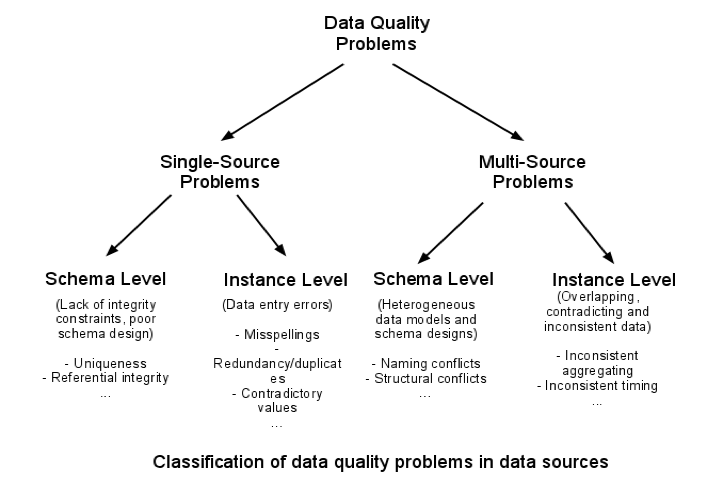
\includegraphics[scale=0.5]{ClassificationData.png}
  \caption{}
\end{center}  
\end{figure}

Nous voyons donc qu’il est possible de séparer les problèmes de qualité de données selon deux origines principales :
\begin{itemize}
\item[-]les problèmes internes à une source de données unique
\item[-]les problèmes liés à des données ayant des sources multiples
\end{itemize}
Il est aussi possible de distinguer deux autres sous-catégories de problèmes liés à la qualité des données :
\begin{itemize}
\item[-]les problèmes liés au modèle de données (le schéma de données)
\item[-]les problèmes liés aux données elles-mêmes (incohérences au niveau des données entre autres)
\end{itemize}
Nous aborderons dans un premier temps les problèmes liés aux sources de données uniques.\\
Les problèmes liés aux modèles de données sont principalement des problèmes liés à de mauvaises définitions du modèle données (violation de contraintes d’intégrité, unicité non respectée, valeurs illégales, etc....).\\
Les problèmes liés aux données elles-même sont quant-à-eux un peu plus variés. Il peut s’agir de problèmes liés à des valeurs manquantes ou erronées (fautes de frappes, d’orthographe, abréviations, erreurs de champs, etc...), à des incohérences entre plusieurs valeurs d’une même données (exemple : ville Paris, et code postal 42000), ou encore à des incohérences entre différentes données (données enregistrées plusieurs fois - et éventuellement de manière légèrement différentes, données incohérentes entre-elles).\\
Il est évident que ces problèmes se retrouvent souvent combinés entre-eux, et ainsi créer des problèmes bien plus complexes.\\
Les meilleurs moyens de résoudre (la plupart) de ces problèmes consiste à introduire un modèle de données fiable et cohérent laissant le minimum de libertés aux données, évitant ainsi un maximum d’erreurs.\\
Nous verrons ensuite les problèmes liés aux sources de données multiples. Ceux si sont sensiblement aggravés en comparaison des problèmes liés aux sources de données uniques, et sont bien plus nombreux.\\
Les problèmes liés aux modèles de données sont assez nombreux. Tout d’abord, l’un des problèmes provient du fait que les schémas de données des multiples sources sont différents.\\
Il faut donc dans premier temps convertir toutes les sources de données vers un schéma unique. Il faut à ce moment là définir deux autres types de problèmes : 
\begin{itemize}
\item[-]les problèmes de nommage : un même nom d’attribut correspondant à plusieurs types d’attributs différents (homonymes, par exemple id) ou plusieurs noms d’attribut correspondant finalement à unique type d’attribut (synonymes, name et nom par exemple).
\item[-]les problèmes structurels : ce sont des problèmes dus à des représentations de la même donnée de manières différentes (pas le même types de données - bool, string -, contraintes d’intégrité différentes, etc...).
\end{itemize}
Les problèmes liés aux données elles-mêmes sont assez similaires aux mêmes problèmes liés aux sources de données uniques (duplicité des données, incohérences, etc...), combinés aux problèmes de représentation différentes des données. Même si ces problèmes de représentation ne semble pas toujours présents au premier abord (même nom d’attributs, même types de données) il faut rester prudent quant à l’exploitation des résultats (interprétation des données différentes par exemple - prix en dollar ou en euro -...).\\
La principale difficulté posée par la présence de sources de données multiples est en fait la difficulté de déterminer quelles sont les données se référant à une même entité réelle.\\
Si la plupart des problèmes liés aux modèles de données peuvent - et doivent dans la mesure du possible - être corrigés en amont, il n’est pas toujours possible de faire de même concernant les problèmes liées aux données elle-mêmes. C’est donc principalement sur ce problème que s’attardent les solutions de data cleaning.\\
Pour résumer, les données, une fois présentées via le même schéma de données, présentent encore des problèmes de cohérence entre-elles.\\
Il faut donc être capable de déterminer ces incohérences et des les corriger. Ce problème peut se décomposer en deux sous-problèmes principaux :
\begin{itemize}
\item[-]déterminer les données se référant à une unique entité du monde réel (record matching, implémenté par la plupart des systèmes de data cleaning)
\item[-]corriger ces données incohérentes, et supprimer les données redondantes (data repairing, ou merge/purge, que seuls quelques systèmes de data cleaning intègrent)
\end{itemize}
Pour le record matching, dans le meilleur des cas, il y a un attribut unique (ou un groupe d’attributs unique) permettant d’identifier clairement les données, et donc de déterminer si deux entrées se réfèrent à la même entité réelle.\\
Cependant, si on ne dispose pas d’attribut permettant d’identifier les données, ou si ces données sont de mauvaise qualité, il est impossible de déterminer si deux entrées se réfèrent à la même entité réelle par de simple comparaison d’attributs.
Il est donc nécessaire d’introduire un système de “fuzzy matching” (correspondance floue ?).\\
Ce système fait intervenir des “règles de correspondance” permettant de déterminer si deux entrées correspondent ou non à la même entité. Ces règles permettent de déterminer le degré de correspondance de deux entrées, souvent exprimé par un chiffre entre 1 et 0.\\
Pour chaque entrées, chaque attribut est pris en compte, avec un poids différent, pour le calcul du degré de correspondance.

\subsection{Recherche sur le sujet}
Les systèmes de data cleaning traitent le record matching et le data repairing en tant que deux processus indépendants et séparés.\\
Cependant, dans, certains cas, ces processus peuvent interagir entre eux et s’aider l’un l’autre. La réparation aide à la “concordance” et la “concordance” aide à la réparation.\\
L’article Interaction between Record Matching and Data Repairing, Wenfei Fa et ali., 2011 propose une solution permettant d’unifier ces deux processus. Chacune des règles utilisées pour le record matching et le data repairing (les Conditional Functional Dependencies, les Conditionals Inclusion Dependencies et les Matching Dependencies) sont unifiées et traitées en tant que processus unique.\\
Cela permet d’améliorer la qualité des données finales.
\section{Les challenges}
\section{Conclusion}
	La gestion et la qualité des données des entreprises sont un problème d'actualité. Une des solutions les plus appliquées aujourd'hui au sein des SI est le Master Data Management. \\
Nous avons présenté la solution d'une part d'un point de vue technologique, puis d'un point de vue fonctionnel auprès des entreprises pour finir sur son intégration au sein des SI.\\
Nous avons conscience que ce n'est pas la seule solution qui réponds au besoin de qualité de données, il existe actuellement des sociétés qui proposent des solutions de nettoyages de données. Cependant le Master Data Management est la solution qui permet au SI d'avoir la meilleure maintenabilité de leurs parcs de données.\\
Le MDM est un concept relativement nouveau et lance de nombreux défis dus à sa complexité. La plus grande complexité vient des modifications des processus de l'entreprise et des issues du processus d'intégration.
\section{Bibliographie}
\paragraph*{}
\textbf{Enjeu de la qualité des données}\\
BRASSEUR, Christophe. Data Management : qualité des données et compétitivité. Paris : Hermès, 2005. 164 p. Management et Informatique. ISBN 2-7462-1210-2
\paragraph*{}
\textbf{Data Cleaning}\\
\url {http://www.lifl.fr/~bonifati/teaching/dq/lucidi/pods08Tutorial.pdf}
\url {http://homepages.inf.ed.ac.uk/sma1/pubs/sigmod2011.pdf}
\url {http://wwwiti.cs.uni-magdeburg.de/iti_db/lehre/dw/paper/data_cleaning.pdf}
\url {http://qdb2011.dia.uniroma3.it/participants/program/p47-GOLAB.PDF}
\paragraph*{}
\textbf{Le MDM}\\
\url {http://www.oracle.com/us/products/applications/master-data-management/018876.pdf}, White Paper, Master Data Management, Oracle\\
\url {http://www-01.ibm.com/software/data/master-data-management/library.html#White\%20papers} ,  White paper, "How Master Data Management Serves the Business", IBM \\
%\newpage
%\begin{figure}[H]
%\begin{center}
% \includegraphics[scale=0.2]{DiagrameSOAPdc4.png}
%  \caption{Protocole de connexion}
%\end{center}  
%\end{figure}

\end{document}
